\section{Private Equilibrium}\label{sec:private}

This section characterizes the entrepreneur's private choices given the subsidy \(s\) and the merger approval probability \(q\).
We proceed in three steps.
First, we solve the entrepreneur's effort choice for each project type.
Second, we characterize private project choice as a function of merger permissiveness.
Third, we derive the entry cutoff and the resulting mass of entrants.

\subsection{Continuation values and effort}

Recall from \eqref{eq:Rj} that, conditional on success, the entrepreneur's continuation payoff under project \(j \in \{I,B\}\) is
\begin{equation}
    R_j(q)
    =
    \pi_E^D(j)
    +
    \beta \bigl[q\Delta_j-k\bigr]_+.
\end{equation}
Because \(\pi_E^D(j)>0\), each \(R_j(q)\) is strictly positive.
Moreover, by Assumption \ref{ass:types}, project \(I\) yields a larger stand-alone payoff,
whereas project \(B\) yields a larger gain from acquisition.

Let
\begin{equation}
    \bar q_j \equiv \frac{k}{\Delta_j},
    \qquad j \in \{I,B\},
\end{equation}
Because Assumption \ref{ass:types} implies \(\Delta_B>\Delta_I>0\), both merger-feasibility thresholds are well-defined, and
\begin{equation}
    \bar q_B < \bar q_I.
\end{equation}
Thus, as merger policy becomes more permissive, the buyout-oriented project becomes merger-feasible strictly before the independence-oriented project does.

The entrepreneur chooses effort \(x \in [0,1]\) to solve
\begin{equation}
    \max_{x \in [0,1]} \;
    xR_j(q)-\frac{x^2}{2}.
\end{equation}
The next assumption ensures that the main-text solution is interior.

\begin{assumption}\label{ass:interior}
For each \(j \in \{I,B\}\) and all \(q \in [0,1]\), the success-contingent return satisfies
\begin{equation}
    0 < R_j(q) < 1.
\end{equation}
In addition, for the equilibrium values of \(s\) and \(q\) considered in the main text,
\begin{equation}
    0
    <
    s + \frac{1}{2}\max\{R_I(q)^2,R_B(q)^2\}
    <
    1.
\end{equation}
\end{assumption}

Under Assumption \ref{ass:interior}, the entrepreneur's optimal effort under project \(j\) is
\begin{equation}\label{eq:xjstar}
    x_j^*(q)=R_j(q),
\end{equation}
and the corresponding ex ante private payoff from entering with project \(j\) is
\begin{equation}\label{eq:Uj}
    U_j(f;s,q)
    =
    s-f+\frac{R_j(q)^2}{2}.
\end{equation}

Since the subsidy \(s\) enters additively in \eqref{eq:Uj}, it affects the entry decision but does not affect the ranking of projects conditional on entry.
Accordingly, project choice is governed entirely by the comparison between \(R_I(q)\) and \(R_B(q)\).

\subsection{Project choice}

To obtain a clean threshold characterization in the main text, we impose a single-crossing condition.

\begin{assumption}\label{ass:singlecross}
The approval probability
\begin{equation}\label{eq:qhat}
    \hat q
    \equiv
    \frac{\pi_E^D(I)-\pi_E^D(B)}
         {\beta(\Delta_B-\Delta_I)}
\end{equation}
satisfies
\begin{equation}
    \hat q \in [\bar q_I,1).
\end{equation}
\end{assumption}

Assumption \ref{ass:singlecross} ensures that any switch toward the buyout-oriented project occurs only once both project types are merger-feasible.
Appendix \ref{app:projchoice} shows that without this restriction, private project choice is characterized by a simple piecewise threshold system.
The same economic mechanism survives in that more general case: project \(I\) is preferred for sufficiently low \(q\), project \(B\) may become attractive already on the intermediate region \([\bar q_B,\bar q_I)\), and once both projects are merger-feasible the payoff difference remains monotone in \(q\).
The maintained assumption is imposed only to keep the main text to a single switching threshold.

\begin{proposition}\label{prop:projectchoice}
Suppose Assumptions \ref{ass:types}--\ref{ass:singlecross} hold.
Then there exists a unique threshold \(\hat q \in [\bar q_I,1)\) such that the entrepreneur's privately optimal project choice is
\begin{equation}
    j^*(q)
    =
    \begin{cases}
        I, & q<\hat q, \\
        \{I,B\}, & q=\hat q, \\
        B, & q>\hat q.
    \end{cases}
\end{equation}
Equivalently, the buyout-oriented project is chosen if and only if merger policy is sufficiently permissive.
\end{proposition}

Proposition \ref{prop:projectchoice} formalizes the key distortion in the model.
A more permissive merger policy does not merely raise the private value of entrepreneurship; it changes the type of project that entrepreneurs pursue.
When \(q\) is low, entrants prefer the project with stronger stand-alone value.
When \(q\) is high, they prefer the project that generates larger gains under acquisition.

Given Proposition \ref{prop:projectchoice}, define the privately relevant continuation value
\begin{equation}\label{eq:Rbar}
    \bar R(q) \equiv \max\{R_I(q),R_B(q)\} = R_{j^*(q)}(q).
\end{equation}
Then the equilibrium effort choice is
\begin{equation}\label{eq:xstar}
    x^*(q)=\bar R(q).
\end{equation}

Under Assumptions \ref{ass:types}--\ref{ass:singlecross}, \(\bar R(q)\) admits the piecewise representation
\begin{equation}\label{eq:Rbarpiece}
    \bar R(q)
    =
    \begin{cases}
        \pi_E^D(I), &
        q < \bar q_I, \\
        \pi_E^D(I)+\beta(q\Delta_I-k), &
        \bar q_I \le q < \hat q, \\
        \pi_E^D(B)+\beta(q\Delta_B-k), &
        q \ge \hat q.
    \end{cases}
\end{equation}
Hence the entrepreneur's optimal effort is flat for low values of \(q\), increases with slope \(\beta\Delta_I\) once the independence-oriented project becomes merger-feasible, and increases more steeply with slope \(\beta\Delta_B\) after the project choice switches to the buyout-oriented type.

\subsection{Entry cutoff and entrant mass}

Using \eqref{eq:Uj}, the entrepreneur enters if and only if
\begin{equation}
    \max\{U_I(f;s,q),U_B(f;s,q)\} \ge 0.
\end{equation}
Under Assumption \ref{ass:interior}, this is equivalent to
\begin{equation}\label{eq:entrycutoff}
    f \le f^*(s,q)
    \equiv
    s + \frac{\bar R(q)^2}{2}.
\end{equation}
Because fixed costs are uniformly distributed on \([0,1]\), the equilibrium mass of entrants is
\begin{equation}\label{eq:nsq}
    n(s,q)
    =
    s+\frac{\bar R(q)^2}{2}.
\end{equation}

The next proposition summarizes the comparative statics of merger permissiveness.

\begin{proposition}\label{prop:entrymonotonicity}
Suppose Assumptions \ref{ass:types}--\ref{ass:singlecross} hold.
Then:

\begin{enumerate}
    \item \(\bar R(q)\) is weakly increasing in \(q\), with
    \begin{equation}\label{eq:dRbardq}
        \frac{d\bar R(q)}{dq}
        =
        \begin{cases}
            0, & q < \bar q_I, \\
            \beta \Delta_I, & \bar q_I < q < \hat q, \\
            \beta \Delta_B, & q > \hat q.
        \end{cases}
    \end{equation}

    \item Equilibrium effort \(x^*(q)\) is weakly increasing in \(q\).

    \item The mass of entrants \(n(s,q)\) is weakly increasing in \(q\), with
    \begin{equation}\label{eq:dndq}
        \frac{\partial n(s,q)}{\partial q}
        =
        \bar R(q)\frac{d\bar R(q)}{dq}
        \ge 0.
    \end{equation}
\end{enumerate}
\end{proposition}

Proposition \ref{prop:entrymonotonicity} yields the first important implication for policy analysis.
A more permissive merger environment can increase startup activity even before subsidies are considered.
But this increase is not neutral with respect to project composition:
once \(q\) crosses \(\hat q\), the marginal entrant is guided by buyout value rather than stand-alone competitive strength.

Figure \ref{fig:continuation_values_calibrated} illustrates the basic private-equilibrium mechanism under the calibration reported in the text.
As merger permissiveness rises, the buyout-oriented project's continuation value eventually overtakes that of the independence-oriented project, generating the switching threshold \(\hat q\).

\begin{figure}[t]
\centering
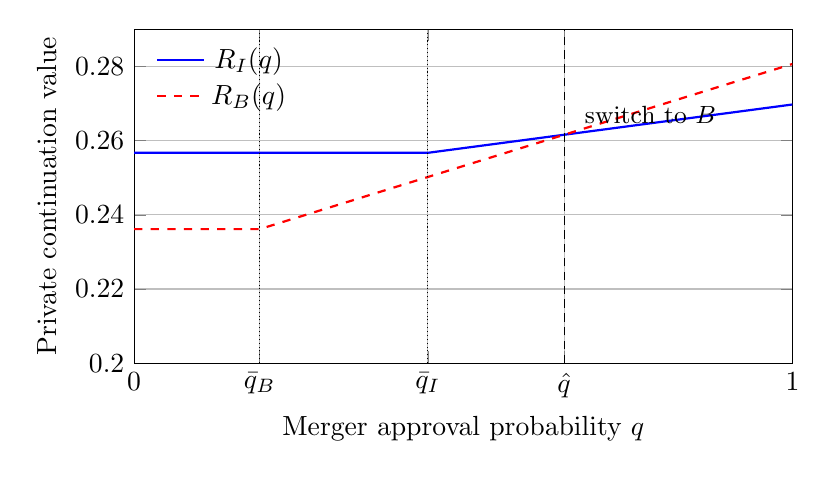
\begin{tikzpicture}
\begin{axis}[
    width=0.82\textwidth,
    height=0.48\textwidth,
    xmin=0, xmax=1,
    ymin=0.20, ymax=0.29,
    xlabel={Merger approval probability \(q\)},
    ylabel={Private continuation value},
    legend style={draw=none, fill=none, at={(0.02,0.98)}, anchor=north west},
    xtick={0,0.1907549041,0.4461335096,0.6531405543,1},
    xticklabels={0,\(\bar q_B\),\(\bar q_I\),\(\hat q\),1},
    ymajorgrids=true,
    xmajorgrids=true
]

\addplot[thick, blue] coordinates {
(0,0.2567111111)
(0.1,0.2567111111)
(0.1907549041,0.2567111111)
(0.3,0.2567111111)
(0.4461335096,0.2567111111)
(0.55,0.25915566668)
(0.6531405543,0.26158313693)
(0.8,0.26503955558)
(1,0.26974666670)
};
\addlegendentry{\(R_I(q)\)}

\addplot[thick, red, dashed] coordinates {
(0,0.2361313702)
(0.1,0.2361313702)
(0.1907549041,0.2361313702)
(0.3,0.24214470712)
(0.4461335096,0.25018854672)
(0.55,0.25590582122)
(0.6531405543,0.26158313696)
(0.8,0.26966693532)
(1,0.28067582660)
};
\addlegendentry{\(R_B(q)\)}

\addplot[densely dotted, black] coordinates {(0.1907549041,0.20) (0.1907549041,0.29)};
\addplot[densely dotted, black] coordinates {(0.4461335096,0.20) (0.4461335096,0.29)};
\addplot[densely dashed, black] coordinates {(0.6531405543,0.20) (0.6531405543,0.29)};

\node[anchor=south west] at (axis cs:0.67,0.262) {\small switch to \(B\)};
\end{axis}
\end{tikzpicture}
\caption{Illustrative private continuation values under the calibration reported in the text. The buyout-oriented project becomes privately optimal only after merger permissiveness passes the switching threshold \(\hat q\).}
\label{fig:continuation_values_calibrated}
\end{figure}

Finally, because \(s\) enters \eqref{eq:Uj} additively, the subsidy affects only the extensive margin.

\begin{corollary}\label{cor:subsidy}
For any given \(q\), the uniform entry subsidy \(s\) does not affect private project choice or effort.
It shifts the entry cutoff one-for-one:
\begin{equation}
    \frac{\partial f^*(s,q)}{\partial s}=1,
    \qquad
    \frac{\partial n(s,q)}{\partial s}=1.
\end{equation}
\end{corollary}

Corollary \ref{cor:subsidy} is useful for what follows.
The local government's uniform subsidy cannot redirect entrepreneurial effort across projects.
It can only expand or contract entry at the privately preferred project margin.
This irrelevance result is specific to a uniform, project-blind subsidy.
If policymakers could condition support on observable project orientation or on realized exit outcomes, project choice could in principle be affected; Section \ref{sec:extensions} illustrates that logic with a second, deliberately reduced-form instrument.
This is precisely why the interaction between merger policy and subsidy policy is central in the subsequent welfare analysis.
